\documentclass[12pt]{article}
\usepackage{graphicx,import}
\usepackage[svgnames]{xcolor} 
\usepackage{fancyhdr}
\usepackage{subfig}
\usepackage{hyperref}
\usepackage{enumitem}
\usepackage{cite}
\usepackage[many]{tcolorbox}
\usepackage{listings }
\usepackage[a4paper, total={6in, 8in} , bottom = 25mm , top = 25mm, headheight = 1.25cm , includehead,includefoot,heightrounded ]{geometry}
\usepackage{afterpage}
\usepackage{amssymb}
\usepackage{pdflscape}
\usepackage{gensymb}
\usepackage{textcomp}
\usepackage{xecolor}
\usepackage{rotating}
\usepackage{pdfpages}
\usepackage[Kashida]{xepersian}
\usepackage[T1]{fontenc}
\usepackage{tikz}
\usepackage[utf8]{inputenc}
\usepackage{PTSerif} 
\usepackage{seqsplit}

\usepackage[edges]{forest}

\usepackage{listings}
\usepackage{xcolor}

\hypersetup{
	colorlinks   = true, %Colours links instead of ugly boxes
	urlcolor     = blue, %Colour for external hyperlinks
	linkcolor    = blue, %Colour of internal links
	citecolor   = red %Colour of citations
}
 
\definecolor{codegreen}{rgb}{0,0.6,0}
\definecolor{codegray}{rgb}{0.5,0.5,0.5}
\definecolor{codepurple}{rgb}{0.58,0,0.82}
\definecolor{backcolour}{rgb}{0.95,0.95,0.92}
 
\NewDocumentCommand{\codeword}{v}{
\texttt{\textcolor{blue}{#1}}
}
\lstset{language=java,keywordstyle={\bfseries \color{blue}}}

\lstdefinestyle{mystyle}{
    backgroundcolor=\color{backcolour},   
    commentstyle=\color{codegreen},
    keywordstyle=\color{magenta},
    numberstyle=\tiny\color{codegray},
    stringstyle=\color{codepurple},
    basicstyle=\ttfamily\normalsize,
    breakatwhitespace=false,         
    breaklines=true,                 
    captionpos=b,                    
    keepspaces=true,                 
    numbers=left,                    
    numbersep=5pt,                  
    showspaces=false,                
    showstringspaces=false,
    showtabs=false,                  
    tabsize=2
}

\lstset{style=mystyle}

\settextfont[Scale=1.2 ,BoldFont={Bahij Nazanin-Bold.ttf} , ItalicFont = {IRNazaninIranic.ttf}]{Bahij Nazanin-Regular.ttf}
\setlatintextfont[Scale = 1.0]{Garamond}
\DefaultMathsDigits 
\DeclareMathSizes{11}{19}{13}{9} 
%\DeclareMathSizes{12}{14.4}{8}{9}





\newenvironment{changemargin}[2]{%
\begin{list}{}{%
\setlength{\topsep}{0pt}%
\setlength{\leftmargin}{#1}%
\setlength{\rightmargin}{#2}%
\setlength{\listparindent}{\parindent}%
\setlength{\itemindent}{\parindent}%
\setlength{\parsep}{\parskip}%
}%
\item[]}{\end{list}}


\definecolor{foldercolor}{RGB}{124,166,198}

\tikzset{pics/folder/.style={code={%
    \node[inner sep=0pt, minimum size=#1](-foldericon){};
    \node[folder style, inner sep=0pt, minimum width=0.3*#1, minimum height=0.6*#1, above right, xshift=0.05*#1] at (-foldericon.west){};
    \node[folder style, inner sep=0pt, minimum size=#1] at (-foldericon.center){};}
    },
    pics/folder/.default={20pt},
    folder style/.style={draw=foldercolor!80!black,top color=foldercolor!40,bottom color=foldercolor}
}

\forestset{is file/.style={edge path'/.expanded={%
        ([xshift=\forestregister{folder indent}]!u.parent anchor) |- (.child anchor)},
        inner sep=1pt},
    this folder size/.style={edge path'/.expanded={%
        ([xshift=\forestregister{folder indent}]!u.parent anchor) |- (.child anchor) pic[solid]{folder=#1}}, inner xsep=0.6*#1},
    folder tree indent/.style={before computing xy={l=#1}},
    folder icons/.style={folder, this folder size=#1, folder tree indent=3*#1},
    folder icons/.default={12pt},
}

\begin{document}


%%% title pages
\begin{titlepage}
\begin{center}
        
\vspace*{0.7cm}

\includegraphics[width=0.4\textwidth]{sharif1.png}\\
\vspace{0.5cm}
\textbf{ \Huge{\emph ‌اندازه‌گیری و کنترل کامپیوتری} }\\
\vspace{0.5cm}
\textbf{ \Large{ تمرین سوم} }
\vspace{0.2cm}
       
 
      \large \textbf{دانشکده مهندسی کامپیوتر}\\\vspace{0.2cm}
    \large   دانشگاه صنعتی شریف\\\vspace{0.2cm}
       \large   ﻧﯿﻢ سال دوم 00-99 \\\vspace{0.2cm}
      \noindent\rule[1ex]{\linewidth}{1pt}
استاد:\\
    \textbf{{جناب آقای دکتر همت‌یار}}


    \vspace{0.15cm}
نام و نام خانوادگی:\\

       
    \textbf{{امیرمهدی نامجو - 97107212}}
\end{center}
\end{titlepage}
%%% title pages


%%% header of pages
\newpage
\pagestyle{fancy}
\fancyhf{}
\fancyfoot{}
\cfoot{\thepage}
\chead{تمرین سوم}
\rhead{\includegraphics[width=0.1\textwidth]{sharif.png}}
\lhead{امیرمهدی نامجو}
%%% header of pages

\KashidaOff


\section*{سوال 4}

$$27 = 1\times 16 + 1\times 8 + 0\times 4 + 1 \times 2 +1 \times 1 = (11011)_2$$

$$0.156 \times 2 = 0.312 \Rightarrow 0$$


$$0.312 \times 2 = 0.624 \Rightarrow 0$$


$$0.624 \times 2 = 1.248 \Rightarrow 1$$


$$0.248 \times 2 = 0.496 \Rightarrow 0$$


$$0.496 \times 2 = 0.992 \Rightarrow 0$$


$$0.992 \times 2 = 1.984 \Rightarrow 1$$


$$0.156 \approx (0.001001)_2$$

$$27.156 \approx (11011.001001)_2$$

مقدار دقیق عدد باینری بدست آمده:
$27 + 2^{-3} + 2^{-6} = 27.140625$
است.
\section*{سوال 8}

$$(\overline{S}\cdot W \cdot R) + (S \cdot \overline{R})$$
\newpage
\section*{سوال 12}


$$360 \mu V / \deg C \times 530 \deg C = 0.190800$$


مدار آن به صورت زیر می‌شود:

\begin{center}
	\includegraphics[width = 1.0 \textwidth]{images/1.png}
\end{center}

یکی از مقاومت ها $100$ فرض شده و مقاومت دیگر با رابطه

$$0.190800 = \frac{100}{100+R} \times 10 \rightarrow R \approx 5141 \Omega$$

تعیین شده است.



\section*{سوال 16}

\begin{enumerate}[label = \harfi*)]
	\item
$100101 \Rightarrow \frac{37}{64} = 0.578125$

$$v_{out} = 10 \times 0.578125 = 5.78128 V $$

\item

$$\Delta V = 10 \times 2^{-6} = 0.15625$$
\end{enumerate}
\section*{سوال 20}

\begin{enumerate}[label = \harfi*)]
	\item
	
	با توجه به بازه داده شده، بازه ولتاژی ما $10$ ولت است و تعداد حالت‌های موردنیاز ما
	$N = \frac{v_{ref}}{\Delta V} = \frac{10}{0.01} = 1000$
	و نزدیک‌ترین عدد توان دو به $1000$ عدد $1024$ یعنی $2^{10}$ است. پس DAC ما $10$ بیتی‌خواهد بود با ولتاژ رفرنس $10$ ولت.
	
	همچنین از آن جایی که باید در زمان $2.5$ میکروثانیه از $0$ تا $1024$ رفته و برگردد، زمان بین عوض شدن خروجی به صورت:
	$\delta t = \frac{2.5 ms}{2048} = 1.221 \mu s$
	خواهد بود.
	
	\item
	
	فلوچارت بدین صورت است (به همراه مقداردهی اولیه به $0$)
	
	
	\begin{center}
		\begin{latin}
		
	
	




\tikzset{every picture/.style={line width=0.75pt}} %set default line width to 0.75pt        

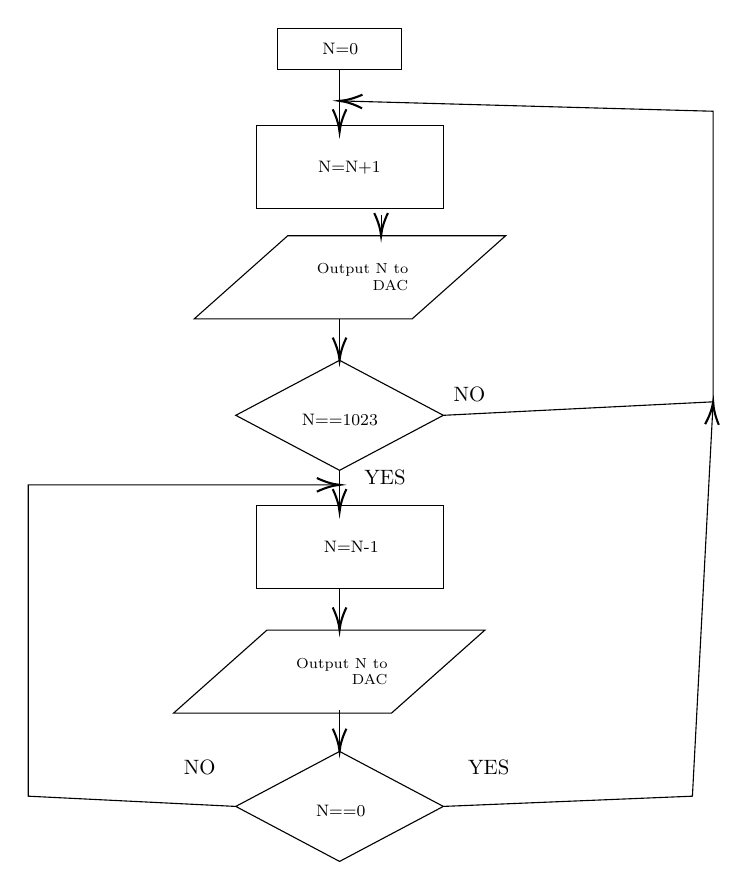
\begin{tikzpicture}[x=0.75pt,y=0.75pt,yscale=-1,xscale=1]
	%uncomment if require: \path (0,441); %set diagram left start at 0, and has height of 441
	
	%Shape: Rectangle [id:dp4147725948146923] 
	\draw   (240,77) -- (330,77) -- (330,117) -- (240,117) -- cycle ;
	%Shape: Parallelogram [id:dp04977048398541495] 
	\draw   (255,130) -- (360,130) -- (315,170) -- (210,170) -- cycle ;
	%Shape: Diamond [id:dp5840879521917679] 
	\draw   (280,190) -- (330,216.5) -- (280,243) -- (230,216.5) -- cycle ;
	%Shape: Rectangle [id:dp44372903004557074] 
	\draw   (250,30) -- (310,30) -- (310,50) -- (250,50) -- cycle ;
	%Shape: Rectangle [id:dp029227429627333157] 
	\draw   (240,260) -- (330,260) -- (330,300) -- (240,300) -- cycle ;
	%Shape: Diamond [id:dp30496314715428463] 
	\draw   (280,378.43) -- (330,404.93) -- (280,431.43) -- (230,404.93) -- cycle ;
	%Shape: Parallelogram [id:dp2246364722176788] 
	\draw   (245,320) -- (350,320) -- (305,360) -- (200,360) -- cycle ;
	%Straight Lines [id:da5961847309553934] 
	\draw    (280,50) -- (280,78) ;
	\draw [shift={(280,80)}, rotate = 270] [color={rgb, 255:red, 0; green, 0; blue, 0 }  ][line width=0.75]    (10.93,-3.29) .. controls (6.95,-1.4) and (3.31,-0.3) .. (0,0) .. controls (3.31,0.3) and (6.95,1.4) .. (10.93,3.29)   ;
	%Straight Lines [id:da6541590619324789] 
	\draw    (300,120) -- (300,128) ;
	\draw [shift={(300,130)}, rotate = 270] [color={rgb, 255:red, 0; green, 0; blue, 0 }  ][line width=0.75]    (10.93,-3.29) .. controls (6.95,-1.4) and (3.31,-0.3) .. (0,0) .. controls (3.31,0.3) and (6.95,1.4) .. (10.93,3.29)   ;
	%Straight Lines [id:da8167788285496835] 
	\draw    (280,170) -- (280,188) ;
	\draw [shift={(280,190)}, rotate = 270] [color={rgb, 255:red, 0; green, 0; blue, 0 }  ][line width=0.75]    (10.93,-3.29) .. controls (6.95,-1.4) and (3.31,-0.3) .. (0,0) .. controls (3.31,0.3) and (6.95,1.4) .. (10.93,3.29)   ;
	%Straight Lines [id:da209615947034002] 
	\draw    (280,243) -- (280,261) ;
	\draw [shift={(280,263)}, rotate = 270] [color={rgb, 255:red, 0; green, 0; blue, 0 }  ][line width=0.75]    (10.93,-3.29) .. controls (6.95,-1.4) and (3.31,-0.3) .. (0,0) .. controls (3.31,0.3) and (6.95,1.4) .. (10.93,3.29)   ;
	%Straight Lines [id:da5285728692950147] 
	\draw    (280,300) -- (280,318) ;
	\draw [shift={(280,320)}, rotate = 270] [color={rgb, 255:red, 0; green, 0; blue, 0 }  ][line width=0.75]    (10.93,-3.29) .. controls (6.95,-1.4) and (3.31,-0.3) .. (0,0) .. controls (3.31,0.3) and (6.95,1.4) .. (10.93,3.29)   ;
	%Straight Lines [id:da26905711690800294] 
	\draw    (280,358.43) -- (280,376.43) ;
	\draw [shift={(280,378.43)}, rotate = 270] [color={rgb, 255:red, 0; green, 0; blue, 0 }  ][line width=0.75]    (10.93,-3.29) .. controls (6.95,-1.4) and (3.31,-0.3) .. (0,0) .. controls (3.31,0.3) and (6.95,1.4) .. (10.93,3.29)   ;
	%Straight Lines [id:da8845729545705618] 
	\draw    (330,216.5) -- (460,210) -- (460,70) -- (282,65.06) ;
	\draw [shift={(280,65)}, rotate = 361.59000000000003] [color={rgb, 255:red, 0; green, 0; blue, 0 }  ][line width=0.75]    (10.93,-3.29) .. controls (6.95,-1.4) and (3.31,-0.3) .. (0,0) .. controls (3.31,0.3) and (6.95,1.4) .. (10.93,3.29)   ;
	%Straight Lines [id:da7553450088634288] 
	\draw    (330,404.93) -- (450,400) -- (459.89,212) ;
	\draw [shift={(460,210)}, rotate = 453.01] [color={rgb, 255:red, 0; green, 0; blue, 0 }  ][line width=0.75]    (10.93,-3.29) .. controls (6.95,-1.4) and (3.31,-0.3) .. (0,0) .. controls (3.31,0.3) and (6.95,1.4) .. (10.93,3.29)   ;
	%Straight Lines [id:da5489856021929083] 
	\draw    (230,404.93) -- (130,400) -- (130,250) -- (278,250) ;
	\draw [shift={(280,250)}, rotate = 180] [color={rgb, 255:red, 0; green, 0; blue, 0 }  ][line width=0.75]    (10.93,-3.29) .. controls (6.95,-1.4) and (3.31,-0.3) .. (0,0) .. controls (3.31,0.3) and (6.95,1.4) .. (10.93,3.29)   ;
	
	% Text Node
	\draw (280,40) node  [font=\footnotesize,xscale=0.75,yscale=0.75] [align=left] {\begin{minipage}[lt]{17.92pt}\setlength\topsep{0pt}
			\begin{flushright}
				N=0
			\end{flushright}
			
	\end{minipage}};
	% Text Node
	\draw (285,97) node  [font=\footnotesize,xscale=0.75,yscale=0.75] [align=left] {\begin{minipage}[lt]{35.38pt}\setlength\topsep{0pt}
			\begin{flushright}
				N=N+1 \ \ 
			\end{flushright}
			
	\end{minipage}};
	% Text Node
	\draw (285,150) node  [font=\scriptsize,xscale=0.75,yscale=0.75] [align=left] {\begin{minipage}[lt]{56.28pt}\setlength\topsep{0pt}
			\begin{flushright}
				Output N to DAC
			\end{flushright}
			
	\end{minipage}};
	% Text Node
	\draw (280,216.5) node  [font=\footnotesize,xscale=0.75,yscale=0.75] [align=left] {\begin{minipage}[lt]{36.3pt}\setlength\topsep{0pt}
			\begin{flushright}
				N==1023
			\end{flushright}
			
	\end{minipage}};
	% Text Node
	\draw (285,280) node  [font=\footnotesize,xscale=0.75,yscale=0.75] [align=left] {\begin{minipage}[lt]{33.34pt}\setlength\topsep{0pt}
			\begin{flushright}
				N=N-1 \ \ 
			\end{flushright}
			
	\end{minipage}};
	% Text Node
	\draw (275,340) node  [font=\scriptsize,xscale=0.75,yscale=0.75] [align=left] {\begin{minipage}[lt]{56.28pt}\setlength\topsep{0pt}
			\begin{flushright}
				Output N to DAC
			\end{flushright}
			
	\end{minipage}};
	% Text Node
	\draw (280,404.93) node  [font=\footnotesize,xscale=0.75,yscale=0.75] [align=left] {\begin{minipage}[lt]{22.68pt}\setlength\topsep{0pt}
			\begin{flushright}
				N==0
			\end{flushright}
			
	\end{minipage}};
	% Text Node
	\draw (334,202) node [anchor=north west][inner sep=0.75pt]  [xscale=0.75,yscale=0.75] [align=left] {NO};
	% Text Node
	\draw (291,242) node [anchor=north west][inner sep=0.75pt]  [xscale=0.75,yscale=0.75] [align=left] {YES};
	% Text Node
	\draw (204,382) node [anchor=north west][inner sep=0.75pt]  [xscale=0.75,yscale=0.75] [align=left] {NO};
	% Text Node
	\draw (341,382) node [anchor=north west][inner sep=0.75pt]  [xscale=0.75,yscale=0.75] [align=left] {YES};
	
	
\end{tikzpicture}
			
		\end{latin}
	\end{center}
	
\end{enumerate}

\section*{سوال 24}

به نظر می‌رسد یک منفی در توان عبارت ورودی صورت داده شده جا افتاده است. وگرنه جواب کلا منفی می‌شود که منطقی نیست.

$$V(t) = 4(1- e^{-t/\tau})$$

$$dV/dt = \frac{4}{\tau} e^{-t/\tau}$$

$$\frac{4}{\tau} e^{-t / \tau} \leq \frac{5.00}{2^{10} \times \tau}$$

بیش‌ترین مقدار سمت چپ به ازای $t=0$ اتفاق می‌افتد.

$$\tau \geq \frac{4 \times 2^{10} \times (44 \times 10^{-6})}{5} = 36.0448 ms$$

پس حداقل مقدار $\tau$ حدود $36ms$ است.



\section*{سوال 28}

عدد $100$ هزار نمونه بر ثانیه به معنی این است که هر نمونه در فاصله $10 \mu s$ گرفته می‌شود. اگر بخواهیم نمونه‌ها را هر $5ms = 5000 \mu s$ بگیریم، بدین معنی است که حدود $4990 \mu s$ را می‌توانیم به ازای هر نمونه صرف پردازش سیگنال و موارد مشابه بکنیم.



\section*{سوال 32}


برای حل این سوال باید بخشی از سوال $31$ را حل کنیم.

برای دما $20$ تا $100$ متناظر با $0.8$ تا $4$ ولت است. برای نگاشت آن به بازه $0$ تا $2.5$ ولت داریم:

$$\left\{\begin{array}{c}
	V = m V_T + V_0\\
	0 = 0.8 m + V_0\\
	2.5 = 4 m + V_0\\
\end{array}\right. \Rightarrow V=0.78125 V_T - 0.625$$


برای فشار $1$ تا $100psi$، بازه مد نظر $0.1$ تا $10$ ولت خواهد بود که برای نظیر کردن آن به $0$ تا $2.5$ ولت داریم:

$$\left\{\begin{array}{c}
	V = m V_P + V_0\\
	0 = 0.1 m + V_0\\
	2.5 = 10 m + V_0\\
\end{array}\right. \Rightarrow V=0.253(V_P - 0.1)$$


برای شار (دبی) بازه $30$ تا $90$ گالن بر دقیقه نظیر $4.5$ تا $13.5$ ولت است که باید به $0$ تا $2.5$ نظیر بشود.

$$\left\{\begin{array}{c}
	V = m V_F + V_0\\
	0 = 4.5 m + V_0\\
	2.5 = 13.5 m + V_0\\
\end{array}\right. \Rightarrow V=0.2778V_F - 1.25$$


با توجه به این موارد داریم:

$$V=0.781 (V_T - 0.8)$$
$$V=0.253(V_P - 0.1)$$
$$V=0.277(V_F -4.5)$$

هر قسمت را به صورت یک مدار جدا با منبع تغذیه $10$ ولت رسم می‌کنیم.

نمودار آن‌ها به صورت زیر می‌شود. در این نمودارها از تقویت‌کننده تفاضلی و دنباله‌کننده ولتاژ استفاده شده است.


\begin{center}
	\includegraphics[width = 0.5 \textwidth]{images/2.png}
\end{center}

\begin{center}
	\includegraphics[width = 0.5 \textwidth]{images/3.png}
\end{center}

\begin{center}
	\includegraphics[width = 0.5 \textwidth]{images/4.png}
\end{center}

\section*{سوال 36}

\begin{enumerate}[label = \harfi*)]
	\item
بازه تغییرات ولتاژی بین
$12 \times -10 = -120 mV$
تا
$+120mV$
است. با توجه به این که ADC داده شده دو قطبی است داریم
$$INT(N) = 2^{12} (\frac{V_{ADC}}{5} + \frac{1}{2})$$

در نتیجه $00$ متناظر با $-10mm$ و معادل با $-2.5 V$ خواهد بود و $FF$ معادل با $10mm$ و معادل با
$V = 5 \times 4095 / 4096 - 2.5 = 2.4988 V$
خواهد بود.

با فرض مبدا گذر بودن ولتاژ
$$V_{out} = 20.833 V_{in}$$

خواهد بود. یعنی مداری با بهره $20.833$ داریم.

با توجه به نویز داده شده، یعنی این نویز معادل خواهد بود با:

$$5 mV \times 20.83 \times \sqrt{2} \approx0.147 V$$

در نتیجه یعنی نویز $\pm 0.147$ روی همه داده‌ها داریم.

این معادل است با
$$\frac{0.147}{(2.5 - (-2.5))} =  \times \frac{2^n}{2^12} \rightarrow n=6.9$$

یعنی در اثر این نویز حدودا $7$ بیت کم ارزش از $12$ بیت می‌توانند دچار تغییر بشوند. 

\item

نرخ نوسان خود سیستم اصلی $1/1.5 = 0.667$ است. در نتیجه فرکانس نویز بالاست و باید یک \lr{Low-Pass Filter} اضافه کنیم. با فرض این که کاهش $99$ درصدی بخواهیم بدهیم داریم:

$$0.01 = 1/\sqrt{1+(60/f_c)^2}\rightarrow f_c = 0.6 Hz$$

با توجه به این موضوع باید ببینم سیگنال اصلی که داریم چقدر کاهش بهره دارد:

$$\frac{V_{out}}{V_{in}} = 1/\sqrt{1+(\frac{0.667}{0.6})^2} = 0.669$$

در نتیجه باید افزایش Gain هم بدهیم.
$20.83/0.669 = 31.14$

در کل نیاز به یک \lr{Low-Pass Filter} و یک تقویت کننده \lr{Noninverting} (یا تقویت کننده‌های دیگر) داریم تا سیگنال مورد نیاز برای ورودی ADC را فراهم کنیم.

با فرض استفاده از خازن $1\mu F$ ای داریم:

$$0.6 = \frac{1}{2 \pi R C} \Rightarrow R = 265.258 k\Omega$$

نتیحه نهایی به صورت شکل زیر خواهد بود:


\begin{center}
	\includegraphics[width = 0.5 \textwidth]{images/5.png}
\end{center}

\end{enumerate}
\section*{سوال 40}


\begin{latin}
\begin{center}
	


\tikzset{every picture/.style={line width=0.75pt}} %set default line width to 0.75pt        

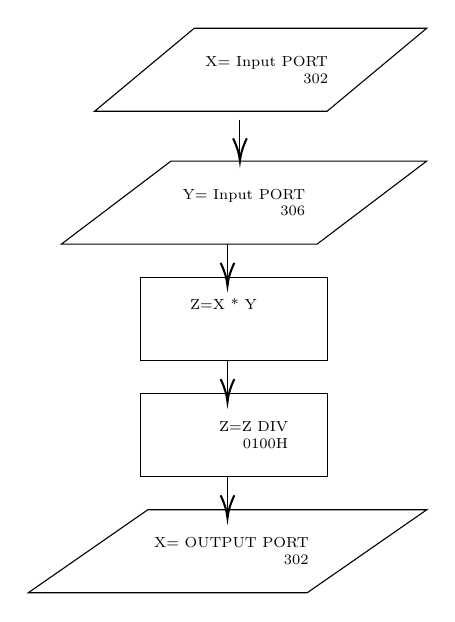
\begin{tikzpicture}[x=0.75pt,y=0.75pt,yscale=-1,xscale=1]
	%uncomment if require: \path (0,441); %set diagram left start at 0, and has height of 441
	
	%Shape: Parallelogram [id:dp04977048398541495] 
	\draw   (256,16) -- (368,16) -- (320,56) -- (208,56) -- cycle ;
	%Straight Lines [id:da8167788285496835] 
	\draw    (278,60) -- (278,78) ;
	\draw [shift={(278,80)}, rotate = 270] [color={rgb, 255:red, 0; green, 0; blue, 0 }  ][line width=0.75]    (10.93,-3.29) .. controls (6.95,-1.4) and (3.31,-0.3) .. (0,0) .. controls (3.31,0.3) and (6.95,1.4) .. (10.93,3.29)   ;
	%Shape: Parallelogram [id:dp6271857977384494] 
	\draw   (244.8,80) -- (368,80) -- (315.2,120) -- (192,120) -- cycle ;
	%Straight Lines [id:da7452195687955427] 
	\draw    (272,120) -- (272,138) ;
	\draw [shift={(272,140)}, rotate = 270] [color={rgb, 255:red, 0; green, 0; blue, 0 }  ][line width=0.75]    (10.93,-3.29) .. controls (6.95,-1.4) and (3.31,-0.3) .. (0,0) .. controls (3.31,0.3) and (6.95,1.4) .. (10.93,3.29)   ;
	%Shape: Rectangle [id:dp9546953047470292] 
	\draw   (230,136) -- (320,136) -- (320,176) -- (230,176) -- cycle ;
	%Straight Lines [id:da8119562657515047] 
	\draw    (272,176) -- (272,194) ;
	\draw [shift={(272,196)}, rotate = 270] [color={rgb, 255:red, 0; green, 0; blue, 0 }  ][line width=0.75]    (10.93,-3.29) .. controls (6.95,-1.4) and (3.31,-0.3) .. (0,0) .. controls (3.31,0.3) and (6.95,1.4) .. (10.93,3.29)   ;
	%Shape: Rectangle [id:dp06721231397338912] 
	\draw   (230,192) -- (320,192) -- (320,232) -- (230,232) -- cycle ;
	%Shape: Parallelogram [id:dp17602028086396815] 
	\draw   (233.6,248) -- (368,248) -- (310.4,288) -- (176,288) -- cycle ;
	%Straight Lines [id:da8933647637306346] 
	\draw    (272,232) -- (272,250) ;
	\draw [shift={(272,252)}, rotate = 270] [color={rgb, 255:red, 0; green, 0; blue, 0 }  ][line width=0.75]    (10.93,-3.29) .. controls (6.95,-1.4) and (3.31,-0.3) .. (0,0) .. controls (3.31,0.3) and (6.95,1.4) .. (10.93,3.29)   ;
	
	% Text Node
	\draw (288,36) node  [font=\scriptsize,xscale=0.75,yscale=0.75] [align=left] {\begin{minipage}[lt]{64.96pt}\setlength\topsep{0pt}
			\begin{flushright}
				X= Input PORT 302
			\end{flushright}
			
	\end{minipage}};
	% Text Node
	\draw (277,100) node  [font=\scriptsize,xscale=0.75,yscale=0.75] [align=left] {\begin{minipage}[lt]{64.96pt}\setlength\topsep{0pt}
			\begin{flushright}
				Y= Input PORT 306
			\end{flushright}
			
	\end{minipage}};
	% Text Node
	\draw (267.5,153) node  [font=\scriptsize,xscale=0.75,yscale=0.75] [align=left] {\begin{minipage}[lt]{37.31pt}\setlength\topsep{0pt}
			\begin{flushright}
				Z=X * Y \ \ \ \ 
			\end{flushright}
			
	\end{minipage}};
	% Text Node
	\draw (275,212) node  [font=\scriptsize,xscale=0.75,yscale=0.75] [align=left] {\begin{minipage}[lt]{52.51pt}\setlength\topsep{0pt}
			\begin{flushright}
				Z=Z DIV 0100H
			\end{flushright}
			
	\end{minipage}};
	% Text Node
	\draw (272,268) node  [font=\scriptsize,xscale=0.75,yscale=0.75] [align=left] {\begin{minipage}[lt]{78.3pt}\setlength\topsep{0pt}
			\begin{flushright}
				X= OUTPUT PORT 302
			\end{flushright}
			
	\end{minipage}};
	
	
\end{tikzpicture}

\end{center}	
	
\end{latin}

فلوچارت اصلی به این شکل می‌شود. می‌توان یکسری مرحله Initialization هم مانند مثال ۲۵ صفحه ۱۶۷ کتاب در نظر گرفت که این جا رسم نشده است.

با فرض این که ADC ما دوقطیب $5$ ولتی باشد و DAC ما هم $10$ ولت تک قطبی بوده و هر دو $8$ بیتی باشند داریم:

$$X:= (V1/5 + 1/2)2^8$$
$$Y:= (V2/5 + 1/2)2^8$$
$$Z:= (V1/5 + 1/2)(V2/5 + 1/2)2^{16}$$
$$Z := Z/2^8 \Rightarrow Z:= (V1/5 + 1/2)(V2/5 + 1/2)2^{8}$$

$$V_{out}:= 10(Z/2^8) = 10(V1/5 + 1/2)(V2/5 + 1/2)$$


قطعا با فرض‌های متفاوت برای ADC و DAC های مورد استفاده، جواب متفاوتی بدست می‌آید و در این مورد سوال چیزی نگفته است.

\section*{سوال 44}

 
\end{document}



